\section{Software-Only Root of Trust}
\textbf{Problem}: How can we achieve DRTM on machines without HW support such as \texttt{SKINIT/SENTER} or SGX?

\textbf{Goal}: Externally verifiable code execution without specialised HW
\subsection{Reflection}
\begin{enumerate}
    \item fill entire memory with random data
    \item clear system state and disable interrupts (secure-ish execution env)
    \item compute hash over memory
    \item return hash and system state to verifier
\end{enumerate}

Verifier checks time it took to compute response, received hash and system state.
To protect against replay attacks (or precomputed results) verifier asks for complete memory hash and two hashes over random intervalls.

\subsection{Genuinity}
Slightly different problem setting: Verifier wants to check code integrity, code execution and that the \textbf{code ran on the machine} it was expected to run on.

\begin{enumerate}
    \item verifier sends checksum code to client
    \item code uses pseudo random access pattern $\xrightarrow{}$ causes cache misses $\xrightarrow{}$ alters performance counters
    \item incorporate those hardware parameters into hash
\end{enumerate}

Simulation of the above would be significantly slower.

\subsection{SWATT}
Rellies on optimal code such that attack can not optimize to gain time.
\begin{enumerate}
    \item verifier sends nonce as seed for random access pattern
    \item walk over memory and compute hash
\end{enumerate}

Attacker would need to check and replace every memory read which reveals its presence. Time consuming task!

Infeasible for large memory. Therefor only use partial memory scans $\xrightarrow{}$ open new attack vectors such as memory copy attacks.

\subsubsection{ICE - Improved Checksum}
Include program counter and data pointer in checksum. For any memory copy attack one will differ from the original one.

\subsubsection{ICE Key Exchange}
\begin{enumerate}
    \item receive challenge from remote party
    \item compute checksum and setup TEE (disable interrupts etc.)
    \item compute secrets in TEE
    \item send back public results
\end{enumerate}

Prevents MITM attacks. Attacker can even know entire memory before protocol runs.

\subsubsection{Pioneer}
\begin{enumerate}
    \item verifiy integrity through SW attestation
    \item setup TEE
    \item setup and run code in TEE
\end{enumerate}
\begin{center}
    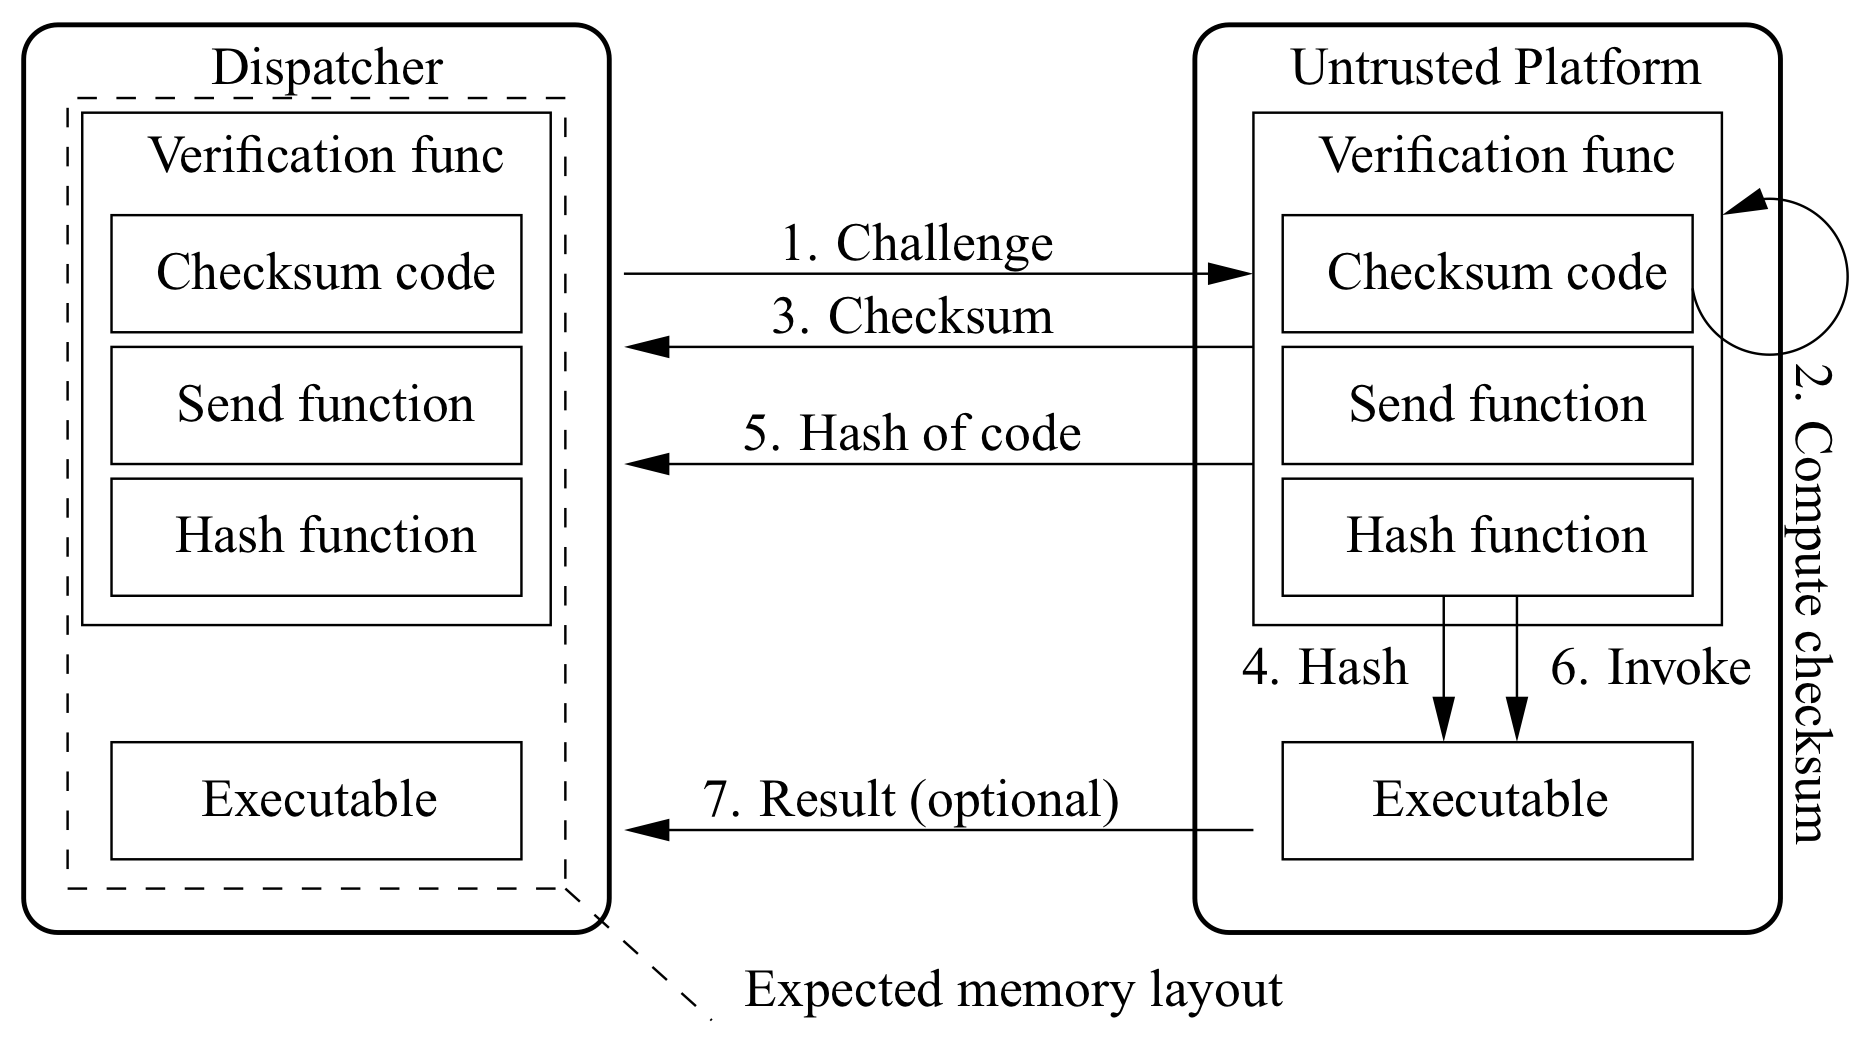
\includegraphics[width=0.8\linewidth]{images/software_attestation-pioneer.png}
\end{center}

Replace interrupt handlers to prevent attacker to interrupt verification function or executable.

\textbf{Trick}: Write checksum to stack, replace handlers right after checksum computation. If attacker causes an interrupt, the interrupt will overwrite stack with checksum $\xrightarrow{}$ attestation fails.
